\chapter{Semi-parametric volatility models}\label{semiparaGarch}

The GARCH model has many advantages. The function form is accessible, and parameters could be easily estimated. If the model assumptions were correct, the estimation is consistent with reality. However, the drawbacks of parametric models are more disgusting. Firstly, a preselected parametric model may not fit unexpected features, due to too restricted or too low dimensional. Secondly, sometimes the regression function seems to be too complicate or difficult to be defined. Thirdly, because different sequence will be witnessed when different conditional distribution is selected in the process of prediction by using parametric models, there will most possibly exist the problem of misspecification, which may result in a excessively high model bias and loss of efficiency, unless the assumed function perfectly matches the true error distribution \citep{Di2011}.

Gourieroux and Monfort had firstly inserted the conditional mean and conditional variance into a nonparametric model, in which the function form is not given. This model can improve the defects of parametric models. Correspondingly, it is less sensitive to model misspecification and can offer a flexible tool in analyzing unknown regression relationships 
\citep{Gourieroux1992}. In nonparametric regression models, both the error distribution and the functional form of the mean function are not pre-specified. It will be more useful when the regression function seems to be very complex or a suitable function form cannot be found \citep{Eubank1993}. However, the nonparametric models lose some functions, which can be realized by parametric models. Due to lack of specific function forms, the parameters of the model cannot be estimated. Furthermore, the model cannot be explained. Excess variable estimates could rise up because of poor consideration of nonparametric models, especially for small sample size. So a new model, semi-parametric model, is proposed.

Semi-parametric model consists of not only the nonparametric part but also parametric part. Semi-parametric GARCH model selects the nonparametric form for the scale function and the parametric part for conditional variance lags. Then it does not need a pre-specified function form and is less sensitive to model misspecification. At the same time, the parametric part can also explain the models \citep{Di2011}.

\section{Semi-GARCH model}

\subsection{Definition of Semi-GARCH model}

Semi-GARCH model combines a smooth scale function with the standard GARCH model:

\begin{equation}
\label{eq:3.1}
Y_{t} = \mu + \sigma(x_{t})\varepsilon_{t},
\end{equation}

where $\mu$ is an unknown constant; $x_{t}=t/n; \sigma(x)>0$ is the nonparametric component, a smooth, bounded scale function; and $\lbrace\varepsilon_{t}\rbrace$ is the parametric component. The conditional variance of $\lbrace\varepsilon_{t}\rbrace$ is assumed to follow a GARCH(p, q) process:

\begin{equation}
\label{equ3.3}
h_{t}=\omega + \sum_{i=1}^{p}\alpha_{i}\varepsilon_{t-i}^{2} + \sum_{j=1}^{q}\beta_{j}h_{t-j},
\end{equation}

where $h_t^{1/2}$ is the conditional standard deviations of the standardized process $\varepsilon_t$; $ \omega>0; \alpha_{1}, \ldots ,\alpha_{p}\geq0$ and $\beta_{1},\ldots,\beta_{q}\geq0$.  To estimate the scale function, $E(\varepsilon_{t}^{8})<\infty$ is assumed to ensure \ref{equ3.3} strictly stationary, which implies in particular that $\sum_{i=1}^p\alpha_i+\sum_{j=1}^q\beta_j<1$ \citep{Feng2004}.

The semi-parametric model provides us a tool to decompose financial risk into an unconditional component $\sigma(x_t)$ , a conditional component $h_{t}^{1/2}$ and the i.i.d. innovations $\eta_{t}$.

\subsection{Estimation of Semi-GARCH model}
\label{subsec3.1.2}
The estimation of Semi-GARCH model can combine the nonparametric estimation of the Y's local variance $v(x)=\sigma^{2}(x)$,with parametric estimation of the unknown parameter vectors $\theta = (\alpha_{0},\alpha_{1},\ldots,\alpha_{p},\beta_{1},\ldots,\beta_{q})$.

At first, the scale function can be estimated by some nonparametric regression approaches without any parametric assumptions. In this model the kernel estimation will be used. If the constant mean $\mu$ is replaced by a sooth function g, we can get a nonparametric regression with scale change and dependence

\begin{equation}
\label{equ3.5}
Y_t= g(x_t)+\sigma(x_t)\varepsilon_t,
\end{equation}

where ${\varepsilon_t}$ is a zero mean stationary process.


Therefore, Equation \ref{eq:3.1} can be transformed into a general nonparametric regression problem at first. Letting $ r_{t}=Y_{t}-\mu$, $X_{t}=r_{t}^{2}$ and $\xi_{t}=\varepsilon_{t}^{2}-1 \geq -1$, which are zero mean stationary time series errors. Then the model \ref{eq:3.1} can be rewritten as 

\begin{equation}
\label{equ3.4}
 X_{t} = v(x_{t} )+ v(x_{t})\xi_{t}.
\end{equation}


Letting $\hat{\mu }=\bar{y}$ and $\hat{x}_{t} = \hat{r}_{t}^{2}$, in which $\hat{r_{t}}$ is then defined by $\hat{r}_{t}=y_{t}-\bar{y}$. A Nadaraya-Watson kernel regression, which has been proposed by Nadaraya (1964) and Watson (1964), is defined by

\begin{equation}
\hat{v}(x)=\frac{\sum_{t=1}^{n}K(\frac{x_t-x}{b})\hat{r}_t}{\sum_{t=1}^{n}K(\frac{x_t-x}{b})}=:\sum_{t=1}^nW_t\hat{r}_t,
\end{equation}

where $W_t$ is the weighting function $W_t= \frac{K(\frac{x_t-x}{b})}{\sum_{t=1}^{n}K(\frac{x_t-x}{b})} $; $K(u)$ is a second order kernel function with compact support [-1,1]; and b is the bandwidth, the size of the weights \citep{Fan1993}. 

According to the above assumptions, the estimator $\varepsilon_{t}$ is now replaced by the standardized residuals

\begin{equation}
\hat{\varepsilon_t }=\hat{r_t}/\hat{\sigma }(x_t)=(y_t-\bar{y})/\hat{\sigma}(x_t). 
\end{equation}

Then the estimator of parametric vector $\theta$ can be obtained by the standard maximum likelihood method, which has been introduced in section 2. A suitable model can also be selected by using other methods, e.g. the akaike information criterion (AIC), the bayesian information criterion (BIC) and etc. \citep{Feng2004}.



\subsection{ Asymptotic properties of $\hat{v}$}
To calculate the asympototic optimal bandwidth, several assumptions must be made:
 \begin{enumerate}
  \item $E(\varepsilon_{t}^{8})<\infty$ ensures the process strictly stationary, and $\eta \sim N(0,1)$\citep{Ling2002}.
  \item The second derivative of $v(x)$ exists and is continuous on $[0,1]$.
  \item The kernel $K(u)$ is a continuous function, which is symmetric around zero and defined in $[-1, 1]$.
  
  \item When the sample volume $n \rightarrow \infty $, the bandwidth $b \rightarrow 0 $ and $nb \rightarrow \infty $. Then both of the bias B and the variance V approaches zero.
 
\end{enumerate}
Define $R(K)= \int K^{2}(u)du$ and $I(K)=\int u^{2}K(u)du$ . Under these assumptions, the asymptotic bias and the asymptotic variance can be obtained.
The asymptotic bias B of $\hat{v}(x)$ is:

\begin{equation}
\label{equ3.6}
B=E[\hat{v}(x)-v(x)] = \frac{I(K)v''(x)}{2}b^{2}+o(b^{2}).
\end{equation}
The asymptotic variance V of $\hat{v}(t)$ can be expressed as:

\begin{equation}
\label{equ3.7}
V=var[\hat{v}(x)]=R(K)\frac{v(x)}{nb}+o(\frac{1}{nb}).
\end{equation}  

From equation \ref{equ3.6} and \ref{equ3.7} we can see that, the bias $B(x)=O(b^2)$ and the variance $V(x)=O(nb)^{-1}$. The bias has the positive correlation with the bandwidth, whereas the variance has the negative correlation with the bandwidth. The higher the $v(x)$, the larger the variance; and the more complex the $v(x)$, the larger the bias.
Then the asymptotic MISE can be calculated by:
\begin{equation}
MISE = \int(B^{2}+V)dt=\frac{I^{2}(K)R(V''(x))}{4}b^{4} + \frac{R(K)}{nb} + o[max(b^{4},\frac{1}{nb})].
\end{equation}
By minimizing the dominant part of the asymptotic MISE, the asymptotically optimal bandwidth of $\hat{v}$ is
\begin{equation}
b=(\frac{R(K)}{I^{2}(K)R(V''(x))})^{1/5}n^{-1/5}.
\end{equation}
When the bandwidth $b=n^{-1/5}$, we can get $\hat{v}(x)=v(x)[1+O_{p}(n^{-2/5})]$ and $MISE=O(n^{-4/5})$ \citep{Gasser1984,Fan1991}.

\subsection{The selection of the bandwidth}
Applying the estimator $\hat{v}$ requires the specification of kernels and bandwidth. Optimal kernels have been obtained analytically. The selection of bandwidth becomes the most important problem when applying nonparametric regression estimators such as kernel estimators. The regression works well, only if the bandwidth is suitable. Because the kernel estimation uses the points around $x_{0}$ to estimate the scale function, a kernel regression is usually biased. The larger the bandwidth, the larger the square bias because further points from $x_{0}$ are used, but the smaller the variance because more observations are used for estimation. The bandwidth should be optimized to balance the variance and bias. The optimal bandwidth is the one, which can minimize the mean squared error (MSE) or mean integrated squared error (MISE) \citep{Gasser1991}. 

There are many methods available to optimize bandwidth, e.g. Cross-Validation (CV), Generalized CV (GCV), plug-in and etc. In this paper, CV and plug-in will be introduced in detail.

\paragraph{Cross-Validation (CV)}

The Cross-Validation method is also called “leave-one-out”. This method estimates the MSE by leaving one observation out at each time point. The main idea of CV is that, the estimation of $v(x_{t})$ is without using $(x_{t},\hat{r_{t}})$, rather assess the quality of the estimation with other observations. 

Define the estimation errors by $\lambda_{-t}=(x_{t},b)=\hat{r}_{t}-\hat{v}^{-t}(x_{t})$. The function to calculate CV is:
\begin{equation}
CV(b) = \sum_{t=1+t_{0}}^{n-t_{0}}\lambda_{-t}^{2}(x_{t},b)=\sum_{t=1+t_{0}}^{n-t_{0}}[\hat{r}_{t}-\hat{v}^{-t}(x_{t})]^{2},
\end{equation}
where $\hat{v}^{-t}(x_t)=\sum_{j=1,j\neq t}^{n}\frac{K(\frac{x_{j}-x_{t}}{b})\hat{r}_{j}}{\sum_{j=1,j \neq t}^{n}K(\frac{x_{j}-x_{t}}{b})}$ is the ``leave-one-out'' estimator of $v(x_{t})$.

Letting $0<h_{min}<h_{max}<1, \bigtriangleup h=(h_{max}-h_{min})/m$, where m is an integer. Then the optimal bandwidth can be obtained by calculating the value of CV at $h=h_{min}, h=h_{min} + \bigtriangleup h, h=h_{min} + 2\bigtriangleup h, \ldots, h=h_{max}$. The optimal bandwidth is the one, at which CV(b) is minimized \citep{Sarda1993}.

Cross-Validation is the most simple method for bandwidth selection and easy to understand. However, this method has large variability, which leads often a suboptimal non-parametric fit of the regression function. For example, the selected bandwidth by CV is often very large. Sometimes the resulted band width can be very small and wrong \citep{Altman1995}. 

\paragraph{Plug-in bandwidth selected method}

In this method, some adapted assumptions are required.


\begin{enumerate}
  \item The function $v(x)$ is strictly positive on [0,1] and exist at least continuous fourth moment.  
  \item $v''$ is estimated with a symmetric fourth order kernel for estimating the second derivative with compacted sup-port [-1,1].
  \item The bandwidth b satisfied $b \rightarrow 0$ and $nb^{5} \rightarrow \infty $ as $n \rightarrow \infty$.
\end{enumerate}

Denote $c_{f}=f(0)$, where $f(\tau)=(2\pi)^{-1}\sum_{k=-\infty}^{\infty}exp(ik\tau)\gamma_{\varepsilon}(k)$ is the spectral density of $\varepsilon_{t}$ with $\gamma_{\varepsilon}(k)$ is the autocovariance function of $\varepsilon_{t}$ . Then the asymptotic optimal bandwidth can be rewritten as 

\begin{equation}
b_{A} =(2\pi c_{f} \frac{R(K)}{I^{2}(K)}\frac{I(v^{2})}{I((v'')^2)})^{1/5}n^{-1/5} = Cn^{-1/5},
\end{equation}

where

\begin{equation}
c_{f}=\frac{E(\varepsilon_{t}^{4})}{3\pi}\frac{(1-\sum_{j=1}^{q}\beta_{j})^{2}}{(1-\sum_{i=1}^{p}\alpha_{i}-\sum_{j=1}^{q}\beta_{j})^{2}}
\end{equation}
 
with the assumption, the functions $\phi(z)=1-\sum_{i=1}^{max(p,q)}\alpha_{i}z^{i}$ and $\varphi(z)=1-\sum_{j=1}^{max(p,q)}\beta_{j}z^{j}$ have no common roots. $\hat{E}(\varepsilon_t^{4})=\sum_{t=1}^{n}\hat{\varepsilon}_{t}^{4}/n$ is a nonparametric estimator of $\varepsilon_{t}^{4}$ \citep{Feng2004}.

This method starts from the asymptotic optimal bandwidth $b_{0}= Cn^{-1/5}$ with C=0.5, then follows iteration process. In the j-th iteration: step 1, calculating $\hat{v}$ and $\hat{\theta}$ with the bandwidth $b_{j-1}$; step 2, calculating $\hat{E}(\varepsilon^{4})$ and $\hat{I}(v)^{2}$ with  $\hat{I}(v)^{2} = \frac{1}{n}\sum_{t=n_{1}}^{n_{2}}\hat{v}(x_{t})^{2}$, where $n_{1}$ and $n_{2}$ denote the integer part of [na] and [n(1-a)] respecyively, in which [a, 1-a] is the compacted support of the mean integrated squared error (MISE). In this calculation, the selected bandwidth is $b_{\varepsilon,j}=b_{v,j}=b_{j-1}^{5/4}$; step 3, calculating $\hat{c}_{f}$ from $\hat{\theta}$ and $\hat{E}(\varepsilon^{4})$; step 4, calculating $\hat{I}((v'')^{2})$, where $\hat{v}''$ is a kernel estimator of  $v''$ with $\hat{I}((v'')^{2})= \frac{1}{n}\sum_{t=n_{1}}^{n_{2}}\hat{v}''(x_{t})^{2}$, in which $\hat{v}''$ is obtained by using the bandwidth $b_{d,j}=b_{j-1}^{5/7}$; step 5, improve $b_{j-1}$ by 
\[ b_{A} =(2\pi \hat{c}_{f} \frac{R(K)}{I^{2}(K)}\frac{\hat{I}(v^{2})}{\hat{I}((v'')^2)})^{\frac{1}{5}}n^{-\frac{1}{5}}; \]

step 6, setting $j=j+1$ and repeating the iteration until a) convergence is reached, where the condition $|b_{j} - b_{j-1}| <1/n$ is used as a criterion for the convergence of $\hat{b}$ ; or b) a given maximal number of iterations has been reached, where the maximal number of iterations is put to be twenty. 

Finally, outputting $\hat{b} = b_{j}$. The asymptotic performance of $\hat{b}$ is quantified by $(\hat{b}-b_{A})/b_{A}=O_{p}(n^{-2/7})+O_{p}(n^{-1/2})$.

The plug-in estimator of the bandwidth has much lower variability than Cross- Validation for a broad variety of situations, including nonsmooth functions \citep{Gasser1991,Feng2004}.

\section{The Semi-APARCH model}
\subsection{Definition of the Semi-APARCH model}

In the Semi-GARCH model, model \ref{equ3.4} is a special case of the model \ref{equ3.5}; and model \ref{equ3.5} can be also written as $r_t= \sigma(x_t)\varepsilon_t$ for $ r_{t}=Y_{t}-\mu$. Now the conditional heteroskedasticity and the scale change can be modeled at the same time.

Denoting $r_{t}= Y_t-\mu,t=1, \ldots,n$ is the logarithmic returns from an asset. According to the above discussion, the Semi-APARCH model is defined as follows:

\begin{equation}
r_{t} = \sigma(x_t)\varepsilon_{t},
\end{equation}

where $\sigma(x_t)$ is a smooth scale function and $\sigma(x_t) >0$; $x_t = t/n$ is the rescaled time; $\varepsilon_{t}$ is the rescaled process \citep{Feng2004}. The conditional variance of the rescaled process $h_{t}$ follows the parametric APARCH model:
  

\begin{equation}
h_{t}^{\delta/2} = \omega + \sum_{i=1}^{p} \alpha_{i}(|\varepsilon_{t-i}|-\gamma_{i}\varepsilon_{t-i})^{\delta} + \sum_{j=1}^{q}\beta_{j}h_{t-j}^{\delta/2},
\end{equation}

where $\omega>0, \delta\geq0, \alpha_{i}\geq0, i=1, \ldots, p, -1<\gamma_{i}<1, i=1, \ldots, p, \beta_{j}\geq0.j=1, \ldots, q$.
The same as introduced in Section \ref{secGarchmodel}, the parametric component should satisfy the assumptions of the parametric APARCH model, such as the stationary condition and etc. $\gamma$ is the leverage parameter and $\delta$ is the parameter for the power term \citep{Ding1993}.


The reason to use Semi-APARCH model rather than the APARCH is that, if the scale function changes over time, the parametric component cannot be estimate consistently from the data, when the non-stationary scale function is not estimated. However, after estimating the nonstationary scale function an approximate stationary process for further analysis can be obtained. When the process follows a parametric model, the semi-parametric framework still works but with some loss of the efficiency \citep{FengYuanhua;Sun2013}.

\subsection{ Estimation of the semi-parametric APARCH model}

From the discussion of kernel regression in section \ref{subsec3.1.2} we can see that, in order to get exact estimation, the sample volume should be larger enough, $n\longrightarrow\infty$. Then $b\longrightarrow0$ and $nb\longrightarrow\infty$. However, the bias is of the order $b^2$ . Therefore, the estimation at the boundary has large bias, which may result in a larger selected bandwidth. This is the called “boundary problem” \citep{Eubank1993}.


In this case, the local linear regression is applied. The mean idea of this regression is that, $v(x)$ is estimated by using a weighted polynomial. Firstly, $v(x)$ is assumed $(p+1)$ times continuously differentiable, where $p\geq1$. Around a point $x_0$, there is 
\[v(x)=v(x_0)+v'(x_0)(x-x_0)+1/2v''(x_0)(x-x_0)^2+...+1/p!v^{(p)}(x_0)(x-x_0)^p+O[(x-x_0)^{p+1}].\]
Then $\hat{\alpha}_0(x_0)$, $\hat{\alpha}_1(x_0)$, $\hat{\alpha}_2(x_0)$,..., $\hat{\alpha}_p(x_0)$ can be obtained by minimizing the locally weighted least squares 
\[Q(x_0)= \sum_{i=1}^n[r_i-\alpha_0(x_0)-\alpha_1(x_0)(x_i-x_0)-\alpha_2(x_0)(x_i-x_0)^2-...-\alpha_p(x_0)(x_i-x_0)^p]^2K(\frac{x_i-x_0}{b})\]

with a kernel $K(u)$. An estimator of $v^{(t)}(x_0)$ can be written as $\hat{v}^{(t)}(x_0)=t!\hat{\alpha_t}(x_0)$ for $t\leq p$ by Taylor's formula (Fan 1993). Then the asymptotic bias and variance are defined by
\[E [ \hat {v}^{(t)}(x_0)-v^{(t)}(x_0)]\approx b^{(k-t)}\frac{v^{(t)}(x_0)\beta}{k!}\]
and
\[var[\hat{{v}^(t)(x_0)}]= \frac{nb^{1+2t}}{h},\]

respectively, where $\beta\neq0$ is a constant. The bias at the boundary stays automatically of the same order as in the interior, without use of specific boundary kernels. This method can solve the boundary problem partly \citep{fan1997}.

There is also another different from the kernel regression in this case. The scale function $v(x)$ is estimated from $|r_t|^d$ with d=1, instead of taking the square root of $\hat{•v}^2(x)$ , which is estimated from $r_t^2$ . The reason of setting d=1 is that ensuring the existence of the fourth order moment of $\varepsilon_{t}$. However, the scale function estimated from $|r_t|$ is an estimation of another function $g(x)$ rather than $v(x)$. Letting $c_1=E(|\varepsilon_{t}|)\neq 1$ , we have $g(x)=c_1v(x)$ and $v(x)=g(x)/c_1$. Then the local linear estimation is used to estimate the scale function.

The local linear estimator $\hat{g}(x)=\hat{a}_0$ at $0\leq x \leq 1$ can be obtained by minimizing

\begin{equation}
Q=\sum_{t=1}^{n}[|r_t|-a_0-a_1(x_t-x)]^2K(\frac{x_t-x}{b}).
\end{equation}

The optimal bandwidth for estimating $g(x)$ is different from the one for estimating $v^2(x)$. In this method a fully data-driven algorithm is used, which is the adapted iterative plug-in idea with a starting bandwidth selected by the cross-validation method. When sample size is small and a small bandwidth is selected, the local linear estimator may lead to negative results. To ensure the non-negativity, the final estimator $\hat{g}_f(x)$ is assumed to be $\hat{g}_f(x)=|\hat{g}(x,d)|$ . Letting $\hat{\varepsilon}_{1,t}=r_t/\hat{g}_f(x)\approx c^{-1}\hat{\varepsilon}$ and assuming $E(\varepsilon_t^4)$ is finite, then the consistent estimate of is
\[\hat{c}_1=[\frac{1}{n}\sum_{t=1}^n\hat{\varepsilon}_{1,t}^2]^{-1/2}.\]

the estimation of $v(x)$ can be obtained by
\[\hat{v}(x_t)=\hat{c}_1^{-1}\hat{g}_f(x_t).\]

Then the estimation of $\varepsilon_t$ can defined as $\hat{\varepsilon}_t=r_t/\hat{v}(x_t)$ . The unknown parameters of a chosen APARCH model can be estimated by approximate conditional maximal likelihood method. AIC or BIC can be used to select a suitable model \citep{FengYuanhua;Sun2013}.

\section{Semi-EGARCH and Semi-CGARCH models}
Based on the semi-parametric GARCH and APARCH models above, the semi-parametric EGARCH and CGARCH models can be defined, which are not introduced in other literatures yet.

The general definition of the semi-EGARCH and semi-CGARCH models, the same as the semi-APARCH model, is composed of the scale function and the conditional heteroscedasticity:

\begin{equation}
r_{t} = \sigma(x_{t})\varepsilon_{t},
\end{equation}
where $r$ is the return process; $\sigma(x_{t})>0$ is the scale function; $x_{t}$ are the rescaled times; and $\varepsilon_{t}$ are the standard residuals with the zero mean and unit variance. 

Different from the semi-APARCH model, the conditional variance of  follows the parametric exponential GARCH model, which was introduced by Nelson in 1991:

\begin{equation}
ln(h_t) =\omega + \sum_{i=1}^p(\alpha_i\eta_{t-i}+\gamma(|\eta_{t-i}|-E|\eta_{t-i}|))+\sum_{j=1}^q\beta_jln(h_{t-j}).
\end{equation}

The assumptions of this parametric component approximate to the parametric exponential GARCH model.

For semi-CGARCH model, the general definition is also the same as the equation (3.17). However, the conditional variance $h_t$ is assumed to follow the parametric component GARCH model, which is introduced by Lee and Engle in 1999:

\begin{equation}
h_{t}=q_{t}+\sum_{i=1}^{p}\alpha_{i}(\varepsilon_{t-i}^{2}-q_{t-i}) + \sum_{j=1}^{q}\beta_{j}(h_{t-j}-q_{t-j}),
\end{equation}

and

\begin{equation}
q_{t} = \omega + \rho q_{t-1} +\varphi(\varepsilon_{t-1}^{2}-h_{t-1}),
\end{equation}

in which $q_{t}$ is the permanent component of the conditional variance and $(h_{t-j} - q_{t-j})$ is the transitory component of the conditional variance; and the parametric specification's assumption of stationary $0<(\alpha + \beta) < \rho <1, 0<\varphi<\beta, \alpha >0, \beta>0, \omega >0 $ should be satisfied \citep{0-19-829683-5,Ghalanos2014}.


%
%\section{Tables and Figures Sample}
%\begin{table}[!h]
% \small
% \caption{Estimated coefficients of the APARCH - norm models for Sap index at open}
% \label{tabValues}
% \centering
% \vspace{2ex}
%
%\resizebox{\textwidth}{!}{ % compress table
% 
%\begin{tabular}{ccc|cc|cc|cc}
%\toprule
%\multirow{2}{*}{} &
%\multicolumn{2}{c|}{APARCH(1,1)} &
%\multicolumn{2}{c|}{APARCH(1,2)} &
%\multicolumn{2}{c|}{APARCH(2,1)} &
%\multicolumn{2}{c}{APARCH(2,2)} \\
%\cline{1-3}\cline{4-5}\cline{6-7}\cline{8-9}
%
%& m{Coeff}  & s.e. & Coeff  & s.e. & Coeff   & s.e.  & Coeff  & s.e. \\
%\midrule
%\hline
%$\mu$  & 0.012459 & 0.013555 & 0.0124602 & 0.01356 & 0.011818 & 0.013940 & 0.012812 & 0.013729  \\
%\hline
%$\omega$  & 0.050010 & 0.006252 & 0.0500216 & 0.00687 & 0.054857 & 0.007283 & 0.097006 & 0.012668 \\
%\hline
%$\alpha_1$   & 0.076004 & 0.006336 & 0.0760131 & 0.00838 & 0.058272 & 0.011220 & 0.052233 & 0.009390 \\
%\hline
%$\alpha_2$   & & & & & 0.021706 & 0.011395 & 0.086890 & 0.008718\\
%\hline
%$\gamma_1$   &1&0.005733 & 0.99999999 &0.00572 &1 & 0.007523 & 1 & 0.009469\\
%\hline
%$\gamma_2$   & & & & &1 & 0.023297&1&0.011564\\
%\hline
%$\beta_1$  & 0.889283&0.009774&0.88929646& 0.09400 &0.879062&0.01205&0.098934&0.079439\\
%\hline
%$\beta_1$  &  & &0.00000001&0.08676& & &0.687549&0.073186\\
%\hline
%$\sigma_1$  & 1.017673&0.12041&1.01704876&0.1207&1.058141&0.127632&1.069076&0.128453\\
%\bottomrule
%\end{tabular}
%} %end of compress
%
%\end{table}
%
%
%\begin{table}[tb]
%  \caption{A Table with some values}
%  \label{tabValues}
%  \centering
%  \vspace{1ex}
%		\begin{tabular}{l|l|l|l|l}
%			Label & Amount of & \multicolumn{3}{c}{Values}\\
%			& something & Case 1 & Case 2 & Case 3\\
%			\hline
%			\hline
%			X & 100\% & 39.59\% & 86.47\% & 87.82\%\\
%			\hline
%			Y & 100\% & 38.03\% & 84.91\% & 86.26\%\\
%			\hline
%			Z & 71.88\% & 34.78\% & 97.83\% & 97.83\%\\
%			\hline
%		\end{tabular}
%\end{table}
%
%%\begin{figure}[htbp]
%%	\centering
%%		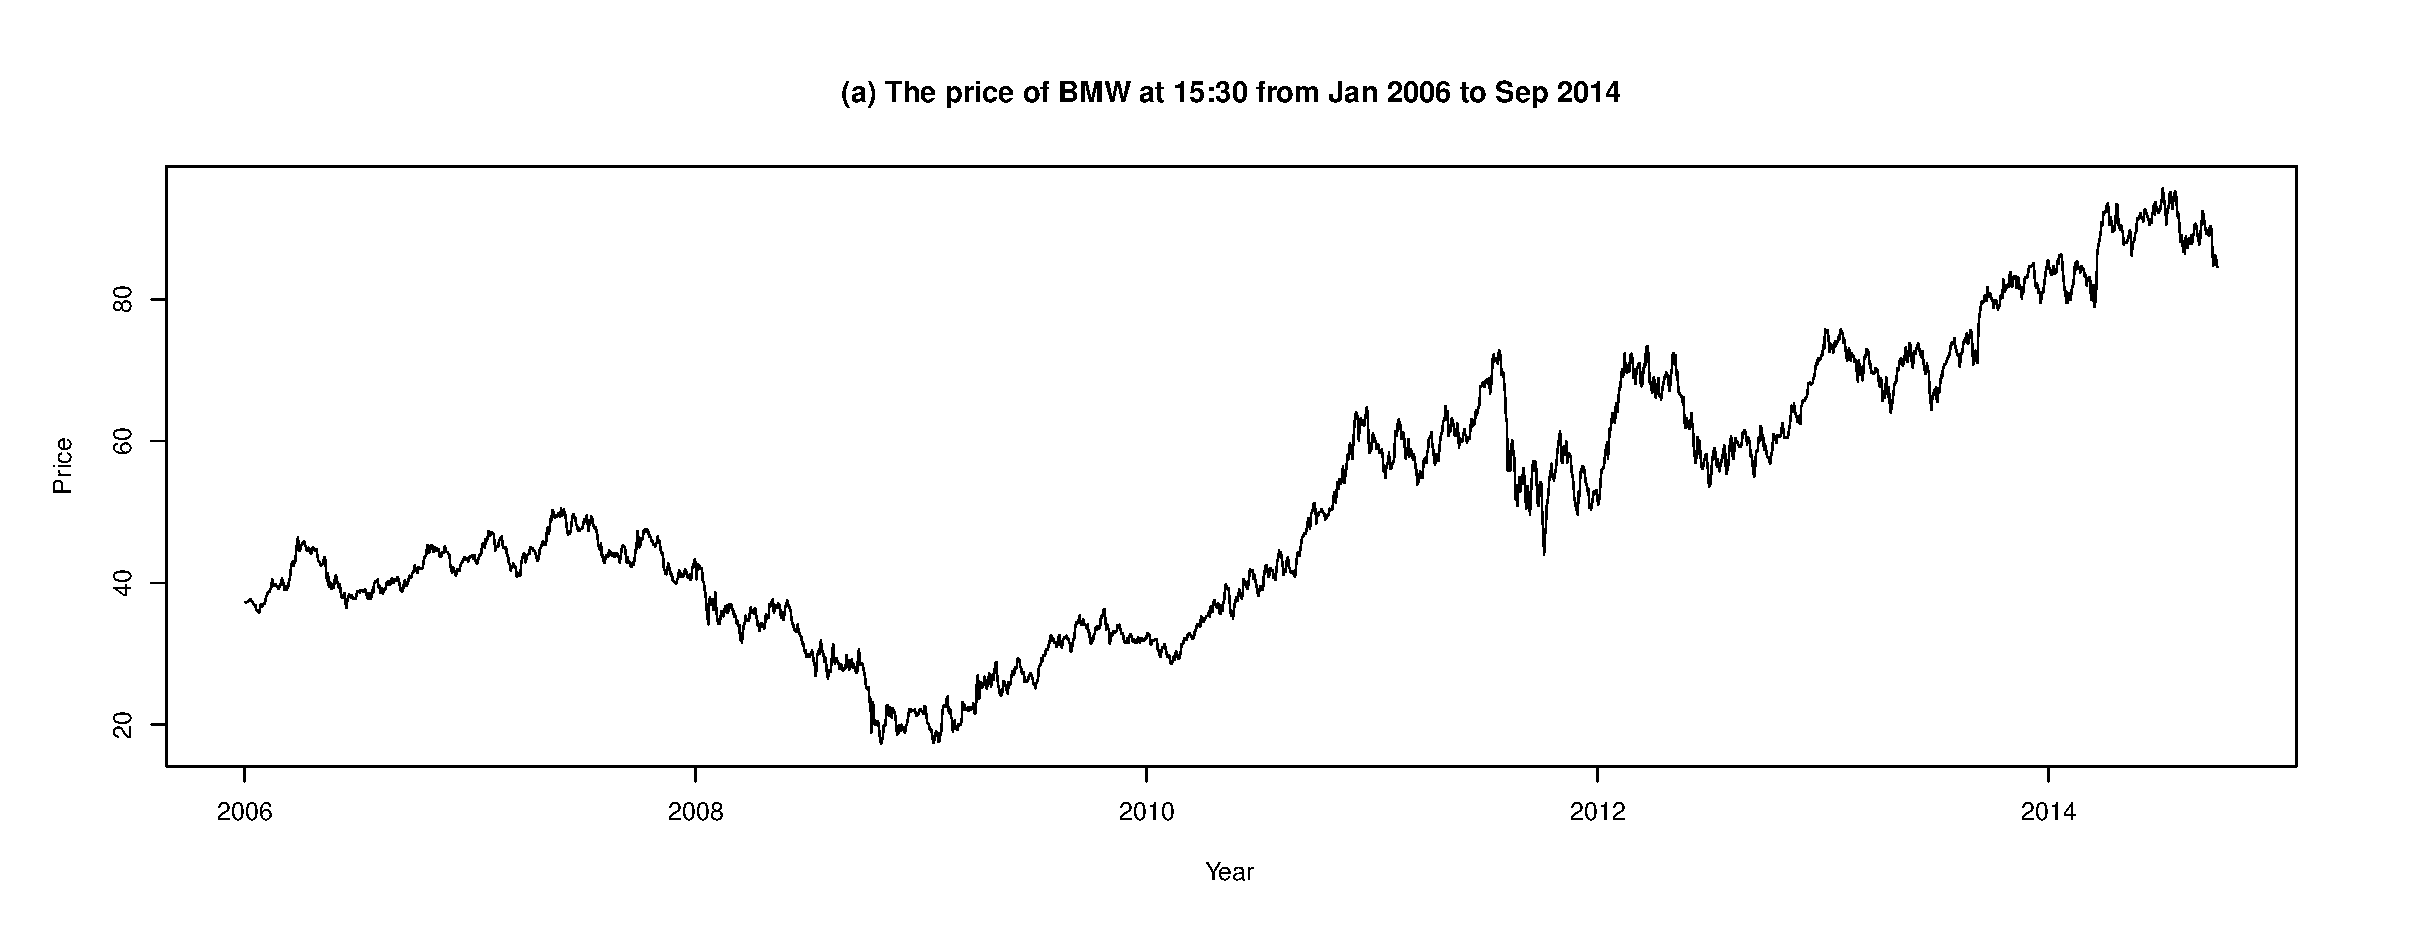
\includegraphics[scale=0.6]{Images/bmw/BMW1530_001.ps}
%%
%%	\label{fig:BMW1530_001}
%%\end{figure}
%
%
%\begin{figure}[t]
%	\centering
%	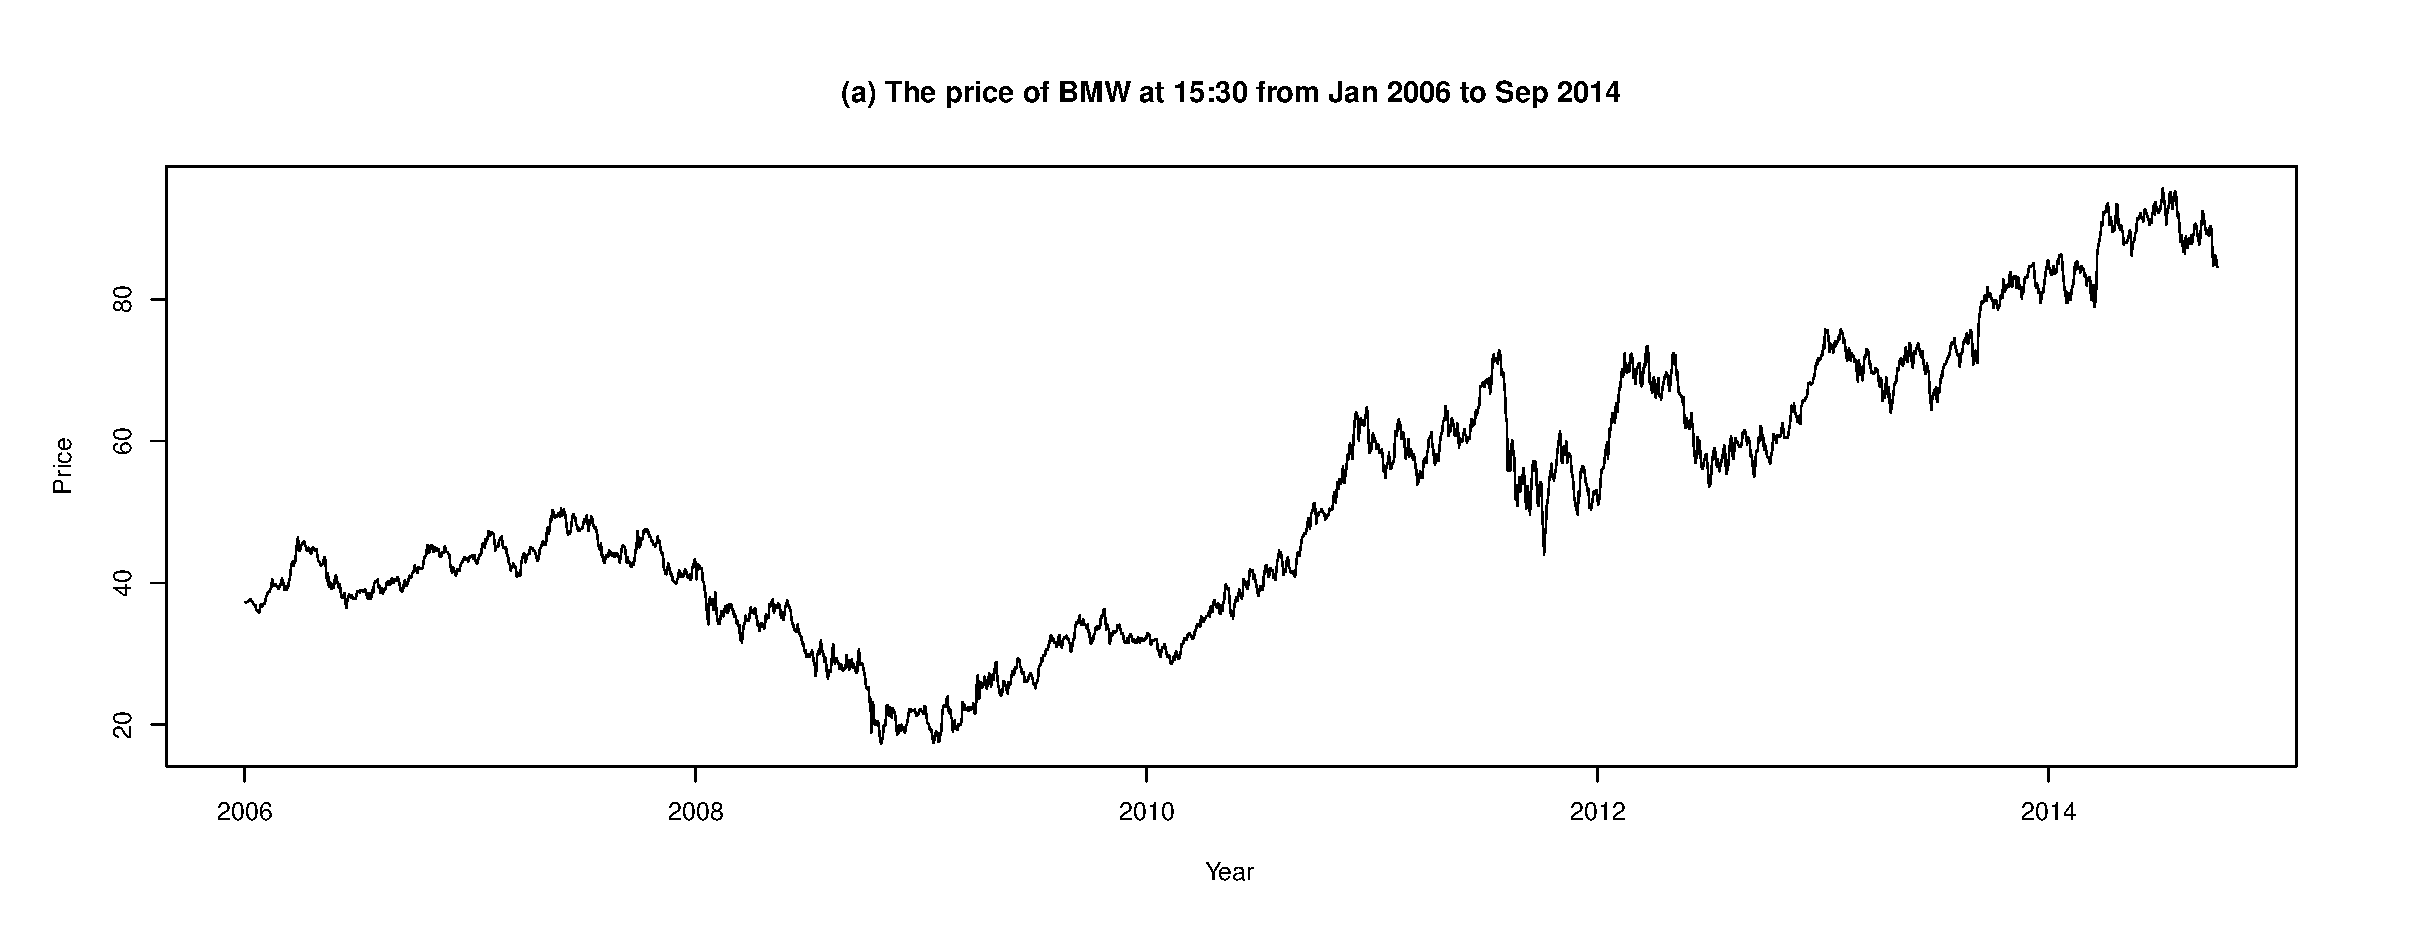
\includegraphics[scale=0.3]{Images/bmw/BMW1530_001}
%	\caption{The price of BMW at 15:30 from Jan 2006 to Sep 2014}
%	\label{fig:BMW1530_001}
%\end{figure}
%
%\begin{figure}[t]
%	\centering
%	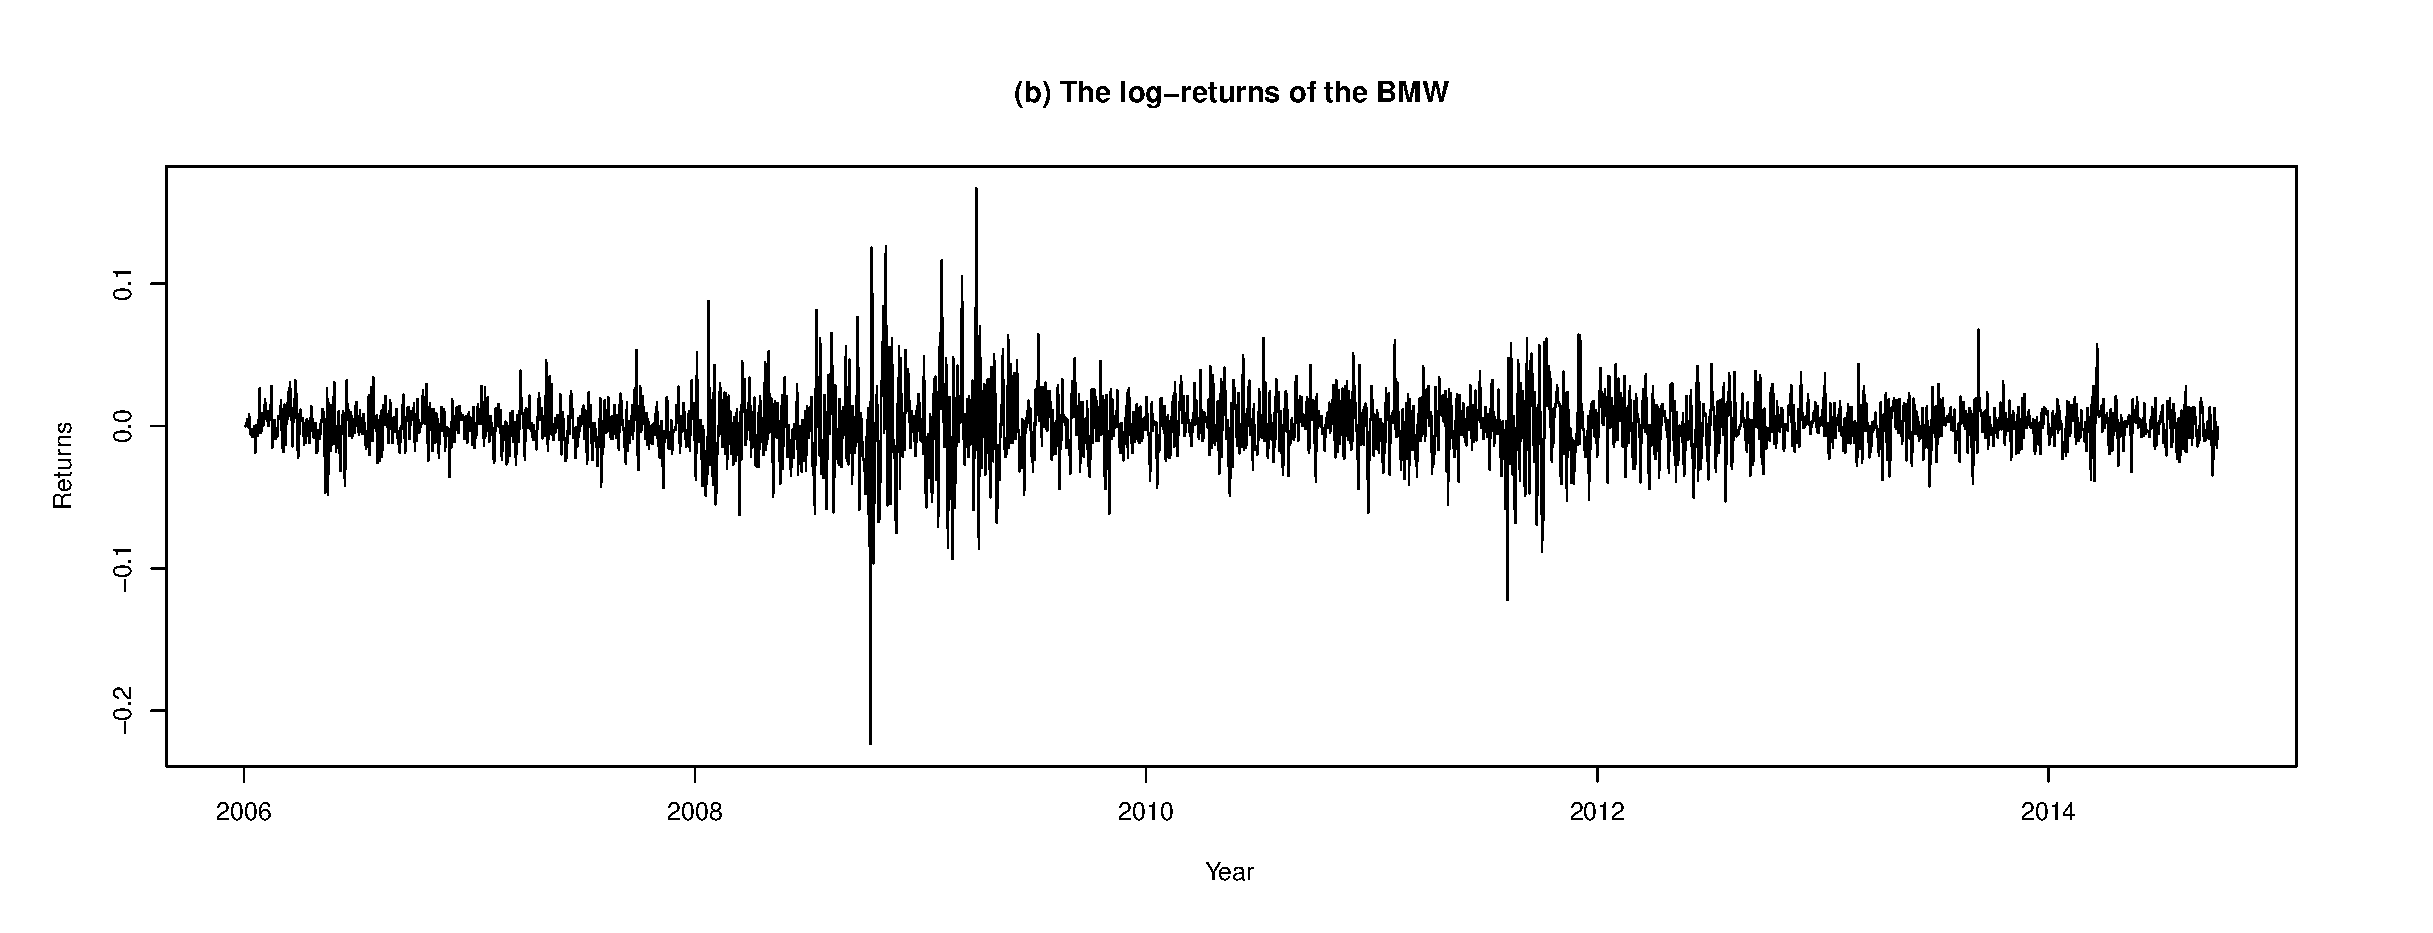
\includegraphics[scale=0.3]{Images/bmw/BMW1530_002}
%	\caption{The log−returns of the BMW}
%	\label{fig:BMW1530_002}
%\end{figure}
%\begin{figure}[t]
%	\centering
%	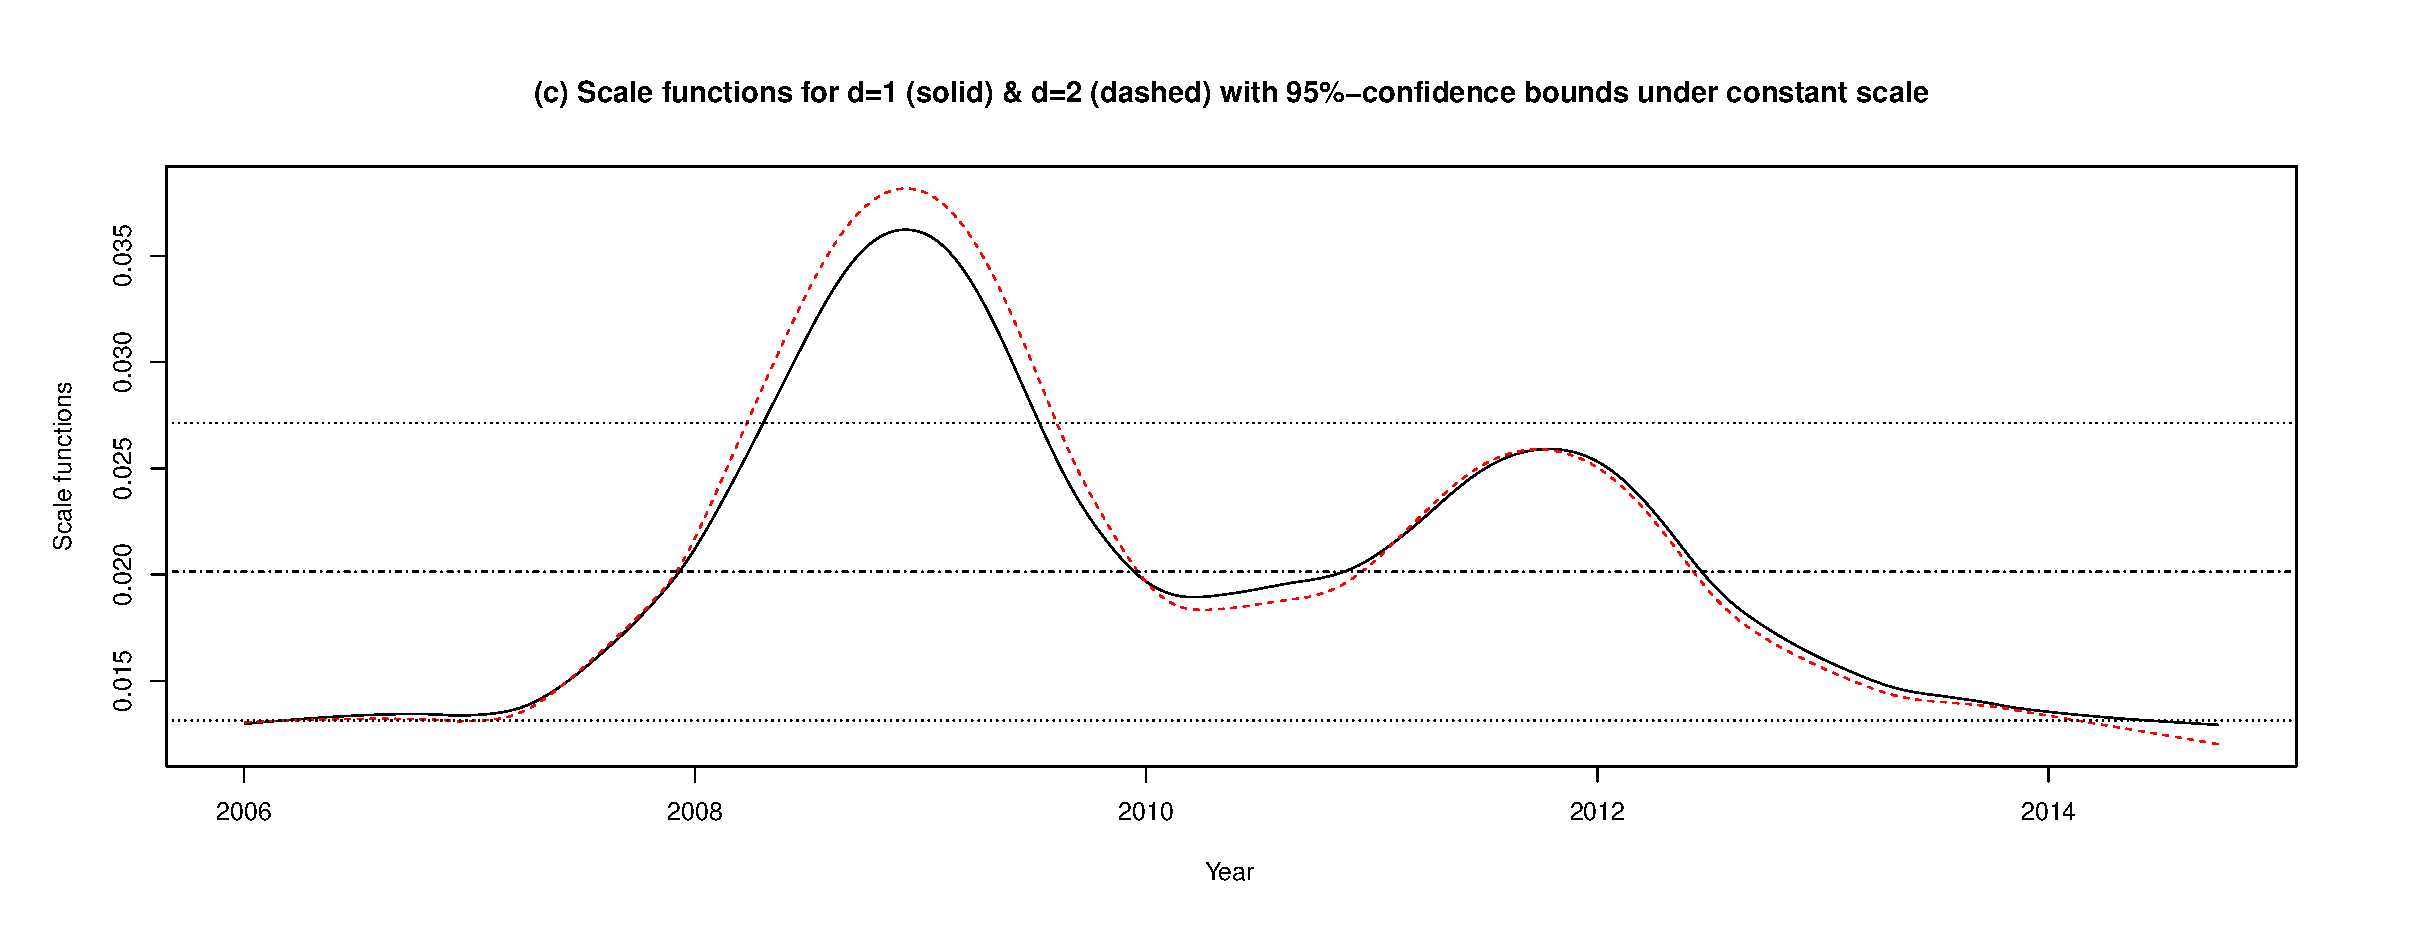
\includegraphics[scale=0.3]{Images/bmw/BMW1530_003}
%	\caption{The price of BMW at 15:30 from Jan 2006 to Sep 2014}
%	\label{fig:BMW1530_003}
%\end{figure}
%\begin{figure}[t]
%	\centering
%	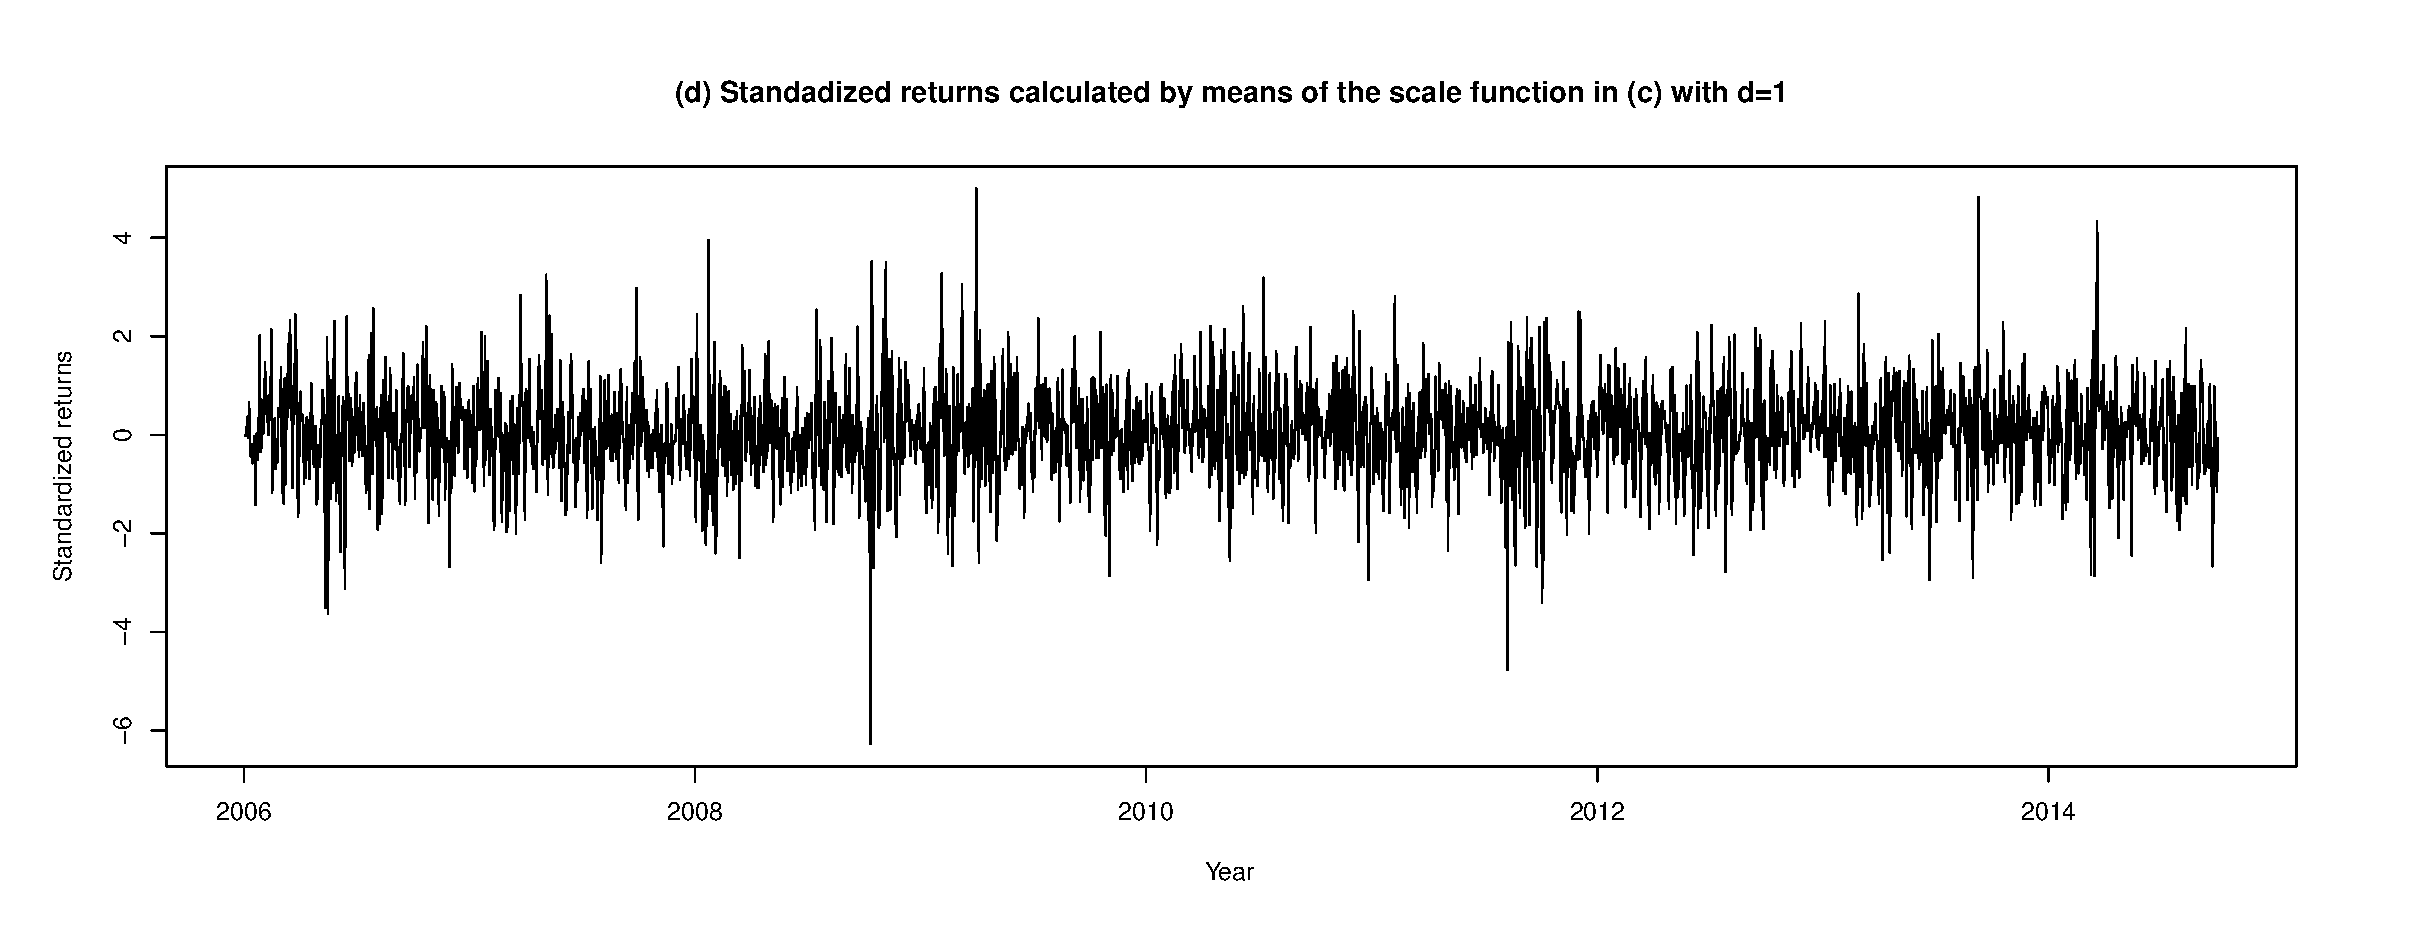
\includegraphics[scale=0.3]{Images/bmw/BMW1530_004}
%	\caption{The price of BMW at 15:30 from Jan 2006 to Sep 2014}
%	\label{fig:BMW1530_004}
%\end{figure}
%
%
